\section{Apparato Sperimentale}

Gli strumenti che abbiamo utilizzato per eseguire questo esperimento sono i seguenti:
\begin{itemize}
	\item{Una bottigla di vetro a cui è applicato un manometro Bourdon di risoluzione di lettura pari a 0.1 bar;}
	\item{Un manometro a U di Torricelli con una risoluzione di lettura di 1 mmHg;}
	\item{Un sistema di raccorderia utilizzato per collegare la pompa a vuoto con la bottiglia e il manometro di Torricelli;}
	\item{Pompa a mano per raggiungere il basso vuoto;}
	\item{Pompa meccanica a membrana doppio stadio (vuoto limite 500 Pa);}
	\item{Cilindri graduati con le seguenti risoluzioni di misura: quello da 1 litro ha una risoluzione di 10 ml, quello da un quarto di litro ha una risoluzione pari a 5 ml ed infine il cilindro graduato da 100 ml ha una rsoluzione di 1 ml;}
	\item{Una bilancia manuale di risoluzione 0.1 g.}
\end{itemize}
%
Nota: %Ci teniamo a specificare che
le indicazioni sulla risoluzione degli strumenti non sono riportate nelle unità di misura del S.I. %sistema internazionale
in quanto abbiamo voluto lasciare le indicazione sulle modalità di misura dello strumento. Nel seguito della relazione tuttavia tutte le misure effettuate e i risultati trovati saranno espressi nelle opportune unità di misura dell'S.I.

\section{Andamento della pressione in funzione del tempo}

Ci proponiamo ora di analizzare l'andamento della pressione interna della bottiglia rispetto a una
variabile discreta, che nel nostro caso è rappresentata dal numero di pompate effettuate
con la pompa a mano. Il risultato è molto simile a quello che si otterrebbe studiando l'andamento
della pressione nel tempo utilizzando una pompa meccanica, da cui il nome del paragrafo.

\subsection{Acquisizione dei dati}

\begin{itemize}
	\item{Abbiamo registrato l'andamento della pressione interna alla bottiglia in funzione del numero di pompate effettuate;}
	\item{Di seguito abbiamo riempito la bottiglia di aria, grazie ad un compressore, fino a raggiungere una pressione
	interna di circa a $3 \cdot 10^5$ \si{\pascal}, e abbiamo valutato l'andamento della pressione interna alla bottiglia
	in funzione del tempo utilizzando la pompa meccanica a membrana a doppio stadio;}
\end{itemize}

\begin{figure}[h!]
    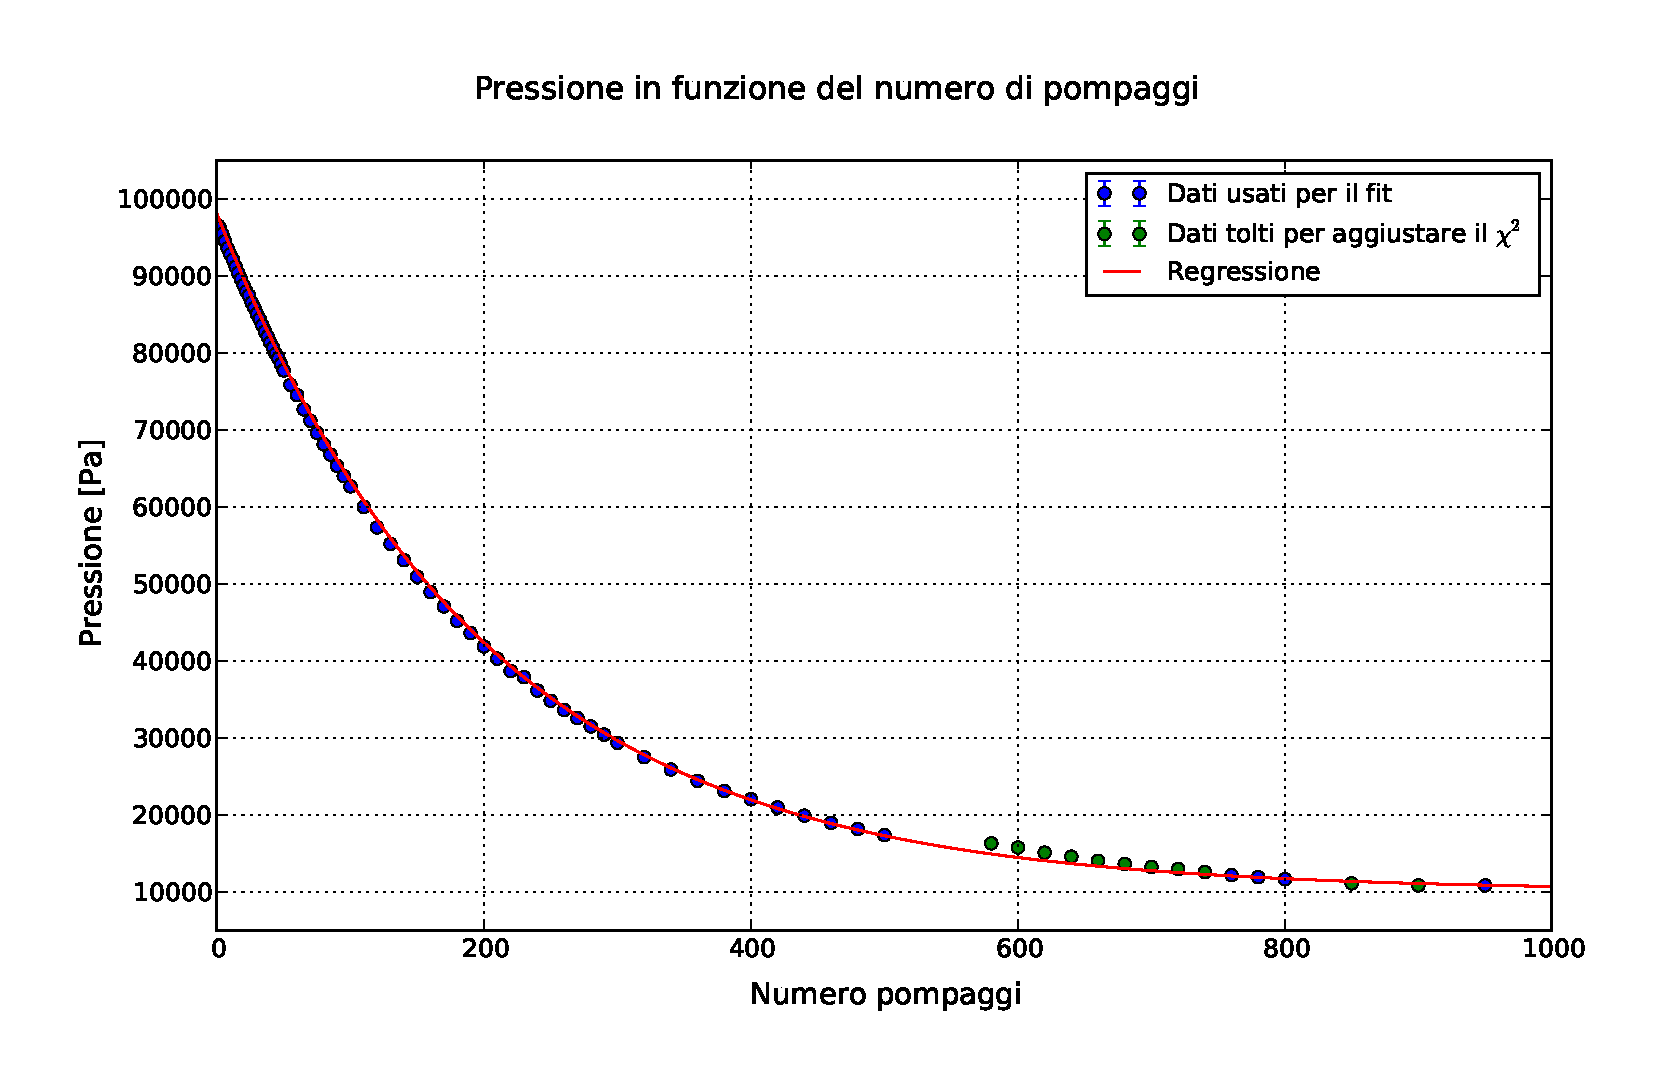
\includegraphics[width=160mm]{graph.pdf}
    \caption{Grafico dei dati ottenuti durante l'esperimento. Il buco presente tra le 500 e le 580 pompate è dovuto ad una perdita d'aria
    che ci ha costretto a fare 60 pompate per tornare al livello precedente. I punti verdi sono stati tolti per aggiustare il $\chi^2$.
    Le barre d'errore sono piccole e non visibili. L'andamento riportato è il risultato della regressione.}
    \label{fig:graph1}
\end{figure}

\subsection{Analisi dei dati}

Graficando i dati raccolti relativi all'andamento della pressione in funzione del numero di pompate effettuate otteniamo
il grafico in Figura \ref{fig:graph1}, che come possiamo notare ha un andamento esponenziale. Inoltre, a parità
il numero di pompate, la variazione di pressione diventa via via più piccola all'aumentare del numero delle
compressioni già effettuate. La pressione tende asintoticamente ad un valore di pressione specifico, il vuoto limite della pompa
da noi utilizzata. Tale valore limite è risultato essere, da calcoli numerici di minimizzazzione del chi quadro, di circa \SI{10000}{\pascal}.

Abbiamo eseguito una regressione, riportata in Figura \ref{fig:graph1}, utilizzando come modello la seguente funzione:

\begin{equation}
    P = P_0 e^{-an} + P_l
\end{equation}
%
dove n è il numero di pompaggi, $P_0$ e $a$ sono costanti e $P_l$ indica la pressione limite.

Col metodo dei minimi quadrati abbiamo ottenuto i valori:

\begin{equation}
    P_0 = 97990 \pm 50 \; \si{\pascal} \qquad a = 5.014 \cdot 10^{-3} \pm 0.006 \cdot 10^{-3} \qquad P_l \simeq \SI{10000}{\pascal}
\end{equation}

Come si vede anche dal grafico in Figura \ref{fig:graph1},
durante l'esperimento si è verificata una perdita attorno alla 500 pompata, che ci ha costretto a scartare alcuni punti.
Comunque abbiamo ottenuto un valore di $P_0$ di poco differente dal valore misurato di $97330 \pm 54 \; \si{\pascal}$.
L'incompatibilità tra i due valori può essere dovuta alla perdita d'aria che ha guastato i nostri dati.

%Per quanto riguarda l'andamento della pressione interna della bottiglia in funzione del tempo, quindi di una variabile che supponiamo continua, i dati da noi ricavati sono riportati nella seguente tabella:

%Il grafico dell'andamento della pressione in funzione del tempo trascorso dall'inizio del processo di svuotamento della bottiglia da parte della pompa meccanica a membrana a doppio stadio è riportato nel grafico sottostante, che come si può notare ha un andamento esponenziale come trovato sopra.

\subsection{Conclusioni prima parte}

Nonostante la perdita di gas, l'esperimento è comunque andato a buon fine, e ci ha permesso di vedere come si comporta
una pompa a vuoto durante la fase di pompaggio.

Per quanto riguarda la parte dell'esperimento con la pompa a membrana, tuttavia, non siamo riusciti ad analizzare l'andamento della pressione in funzione del tempo, quindi di una variabile continua, a causa di una scarsa qualità del video realizzato. Nella ripresa non si vedevano le estremità del manometro di Torricelli, e la lettura del cronometro risultava impossibile. Possiamo però supporre che la curva che avrebbe descritto la pressione in funzione del tempo sarebbe stata, come nel caso precedente, un'esponenziale descrescente, con un andamento asintotico verso la pressione di vuoto limite della pompa a membrana utilizzata.
